\documentclass{article}
\usepackage{graphicx}
\usepackage[utf8]{inputenc}
\usepackage[fleqn]{amsmath}
\usepackage{titling}
\usepackage{graphicx,wrapfig,lipsum}
\usepackage{amssymb}
\usepackage{listings}
\usepackage[font=small,labelsep=none]{caption}
\usepackage{array}% http://ctan.org/pkg/array
\usepackage{lipsum}
\usepackage{subcaption}


\setlength{\droptitle}{-10em}

\title{Project 4}\vspace{-3ex}
\author{Benedicte Allum Pedersen, Emil Helland Broll & Fredrik Oftedal Forr}
\date{\vspace{-5ex}}

\begin{document}
\maketitle


\section{Abstract}

\newpage

\tableofcontents{}

\newpage

\section{Introduction}
In this project we will study the Ising model in two dimensions. This is a model which is used to simulate phase transitions. The model exhibits a phase transition from a magnetic phase to a phase with zero magnetization. The temperature where this phase transition occurs is called the critical temperature, $T_C$. Above this temperature the average magnetization is zero. We study electrons in a lattice which is a binary system because each electron only can take two values, spin up or spin down. \\

The energy we get from the Ising model without an externally applied magnetic field is given by:

\begin{flalign*}
  E = -J \sum_{<kl>}^N S_kS_l
\end{flalign*}

where $s_k, s_l = \pm 1$ and represents classical spin values. N is the total number of spins and J is a coupling constant expressing the strenght of the interactions between neighboring spins. $<kl>$ indicates that we sum over the spins of the nearest neighbors. We apply periodic boundry conditions as well as the Metropolis algorithm. We also assume that we have a ferromagnetic ordering, so $J > 0$.\\

The behavior og physical quantities like the mean magnetization, the heat capacity and the susceptibility can be characterized by a power law behavior when the temperature is near $T_C$. This gives:

\begin{flalign*}
  <M(T)> &\sim (T-T_C)^{\beta},\\
  C_v(T) &\sim |T_C-T|^{\alpha},\\
  \chi(T) &\sim |T_C-T|^{\gamma},
\end{flalign*}

where $\beta = 1/8, \alpha = 0$ and $\gamma = 7/4$. \\

The correlation length is another important physical quantity which can descriped like the ones above. The correlation length, $\varepsilon$, defines the length scale at which the overall properties of a material start to differ from its bulk properties(Jensen, M.). We expect $\varepsilon$ to be of the order of the lattice spacing for $T>>T_C$. As a result of more interactions between the spins as T approaches $T_C$ the correlation length increases as we get closer to $T_C$. Then the divergent behavior of $\varepsilon$ near $T_C$ is

\begin{flalign*}
  \varepsilon(T) \sim |T_C-T|^{-\nu}.
\end{flalign*}

We will always be limited to a finite lattice and $\varepsilon$ will be proportional with the size of the lattice. The behavior of a finite lattice can then be related to the behavior of a infinitely large lattice, so the critical temperature will scale as

\begin{flalign*}
  T_C(L) - T_C(L=\infty) = aL^{-1/\nu}.
\end{flalign*}

If we set $T=T_C$ the mean magnetization, the heat capacity and the susceptibility will be

\begin{flalign*}
  <M(T)> &\sim (T-T_C)^{\beta} \rightarrow L^{-\beta/\nu},\\
  C_v(T) &\sim |T_C-T|^{\alpha} \rightarrow L^{-\alpha/\nu},\\
  \chi(T) &\sim |T_C-T|^{\gamma} \rightarrow L^{-\gamma/\nu}.
\end{flalign*}


\section{Method}

The calculations for the degenerated energies and for the magnetization for 16 different spin configurations is located in the appendix and theese calculations gives us the Table \ref{Tab: EogM} below.

	\begin{table}[h!]
		\caption{: Spinconfigurations grouped by their total energy and magnetization}
			\label{Tab: EogM}
      \centering
		\begin{tabular}{c c c c}
			$\#$ spins up & $\#$ configurations & $E^2$ & M \\
			\hline
			4 & 1 & -8J & 4 \\
			3 & 4 & 0 & 2 \\
			2 & 4 & 0 & 0 \\
			2 & 2 & +8J & 0\\
			1 & 4 & 0 & -2 \\
			0 & 1 & -8J & -4 \\
		\end{tabular}
	\end{table}

We have used the values in Table \ref{Tab: EogM} to calculate, the expectationvalues for the energy and the mean magnetization as well. These values have then been used to calculate the variance for the two physical quantities. The variance for the energi and the mean mean magnetization have respectively been used to calculate the heat capacity $C_v &= \sigma^2_E/k_BT^2$ and the susceptibility $ \chi = \sigma_M^2/k_BT$

\subsection{The Metropolis algorithm}
The Metropolis algorithm uses a propability distribution to obtain a sequence of random samples. In our case it is used to decide if the spins should flip or not. If we have a uniform propability distribution function(PDF), $\omega \in [0,1]$ this is given by:

\begin{flalign*}
    \omega &= \frac{P_i}{P_j} = \frac{P_{new\:state}}{P_{previous\: state}}
     = \frac{e^{-\beta E_i/z}}{e^{-\beta E_j /z}}\\
     \qquad\\
    \omega &= e^{-\beta(E_i-E_j)} = e^{-\beta \Delta E}\\
\end{flalign*}

\noindent where $\Delta E $ is the energy difference between the new and the previous state, $E_i$ and $E_j$. $\beta = 1/k_BT$ and Z is the partition function described in the Appendix(Section 7.2).
If $\omega = 1$ the system will stay at the same place, there will be no change in the spin configuration. If $\omega > 1$ the system will move to a larger propability of spin configurations and if $\omega < 1$ the system move to a smaller propability.

\section{Results}
For a 2 dimensional lattice we need 10 000 Monte Carlo cycles in order to achieve a good agreement, then the mean value of the energy is -7.9864, which is a differnce of 0.007814 from the analytical value. The values described in the sections above are represented in Table \ref{Tab: values} we have set $J/k_BT =\beta J = 1$. The calculations for the analytical values can be found in the Appendix.

{\renewcommand{\arraystretch}{1.5}
\begin{table}[h!]
  \caption{: Analytical and numerical values for T = 1.0, L = 2 and $10^7$ Monte Carlo cycles }
    \label{Tab: values}
    \centering
  \begin{tabular}{c c c c}
    Property & Analytical & Analytical per spin & Numerical per spin \\
    \hline
    $\left<E\right>$ & -7.978586  & -1.994647 & -1.99594\\
    $\left<E^2\right>$ & 63.65786 & 15.91447 &15.9675 \\
    $C_v$ & 0.170865 & 0.042716 & 0.0324227 \\
    $\left<M(T)\right>$  & 0 & 0 & -0.0025167\\
    $\left<|M(T)|\right>$ & 3.991970 & 0.997993 & 0.998647 \\
    $\left<|M(T)|^2\right> $ & 15.962527 & 3.990631 & 3.99323\\
    $\chi$ & 0.026703 & 0.006676 & 0.00202647\\
  \end{tabular}
\end{table}

We have further studied more carefull how many Monte Carlo cycles we need in order to achieve the most likley state for the mean energy and the mean magnetization in a 20 x 20 lattice. Figure \ref{fig:steady_E} shows the results for two different spin matrices, one with all spins up and one random matrix. For the random spin configuration the steady state achives around 200 000 Monte Carlo cycles while for the matrix with all spins up we only need a few cycles.

\begin{figure}
\makebox[\textwidth]{\makebox[1.5\textwidth]{%
\begin{subfigure}{.5\textwidth}
    \centering
    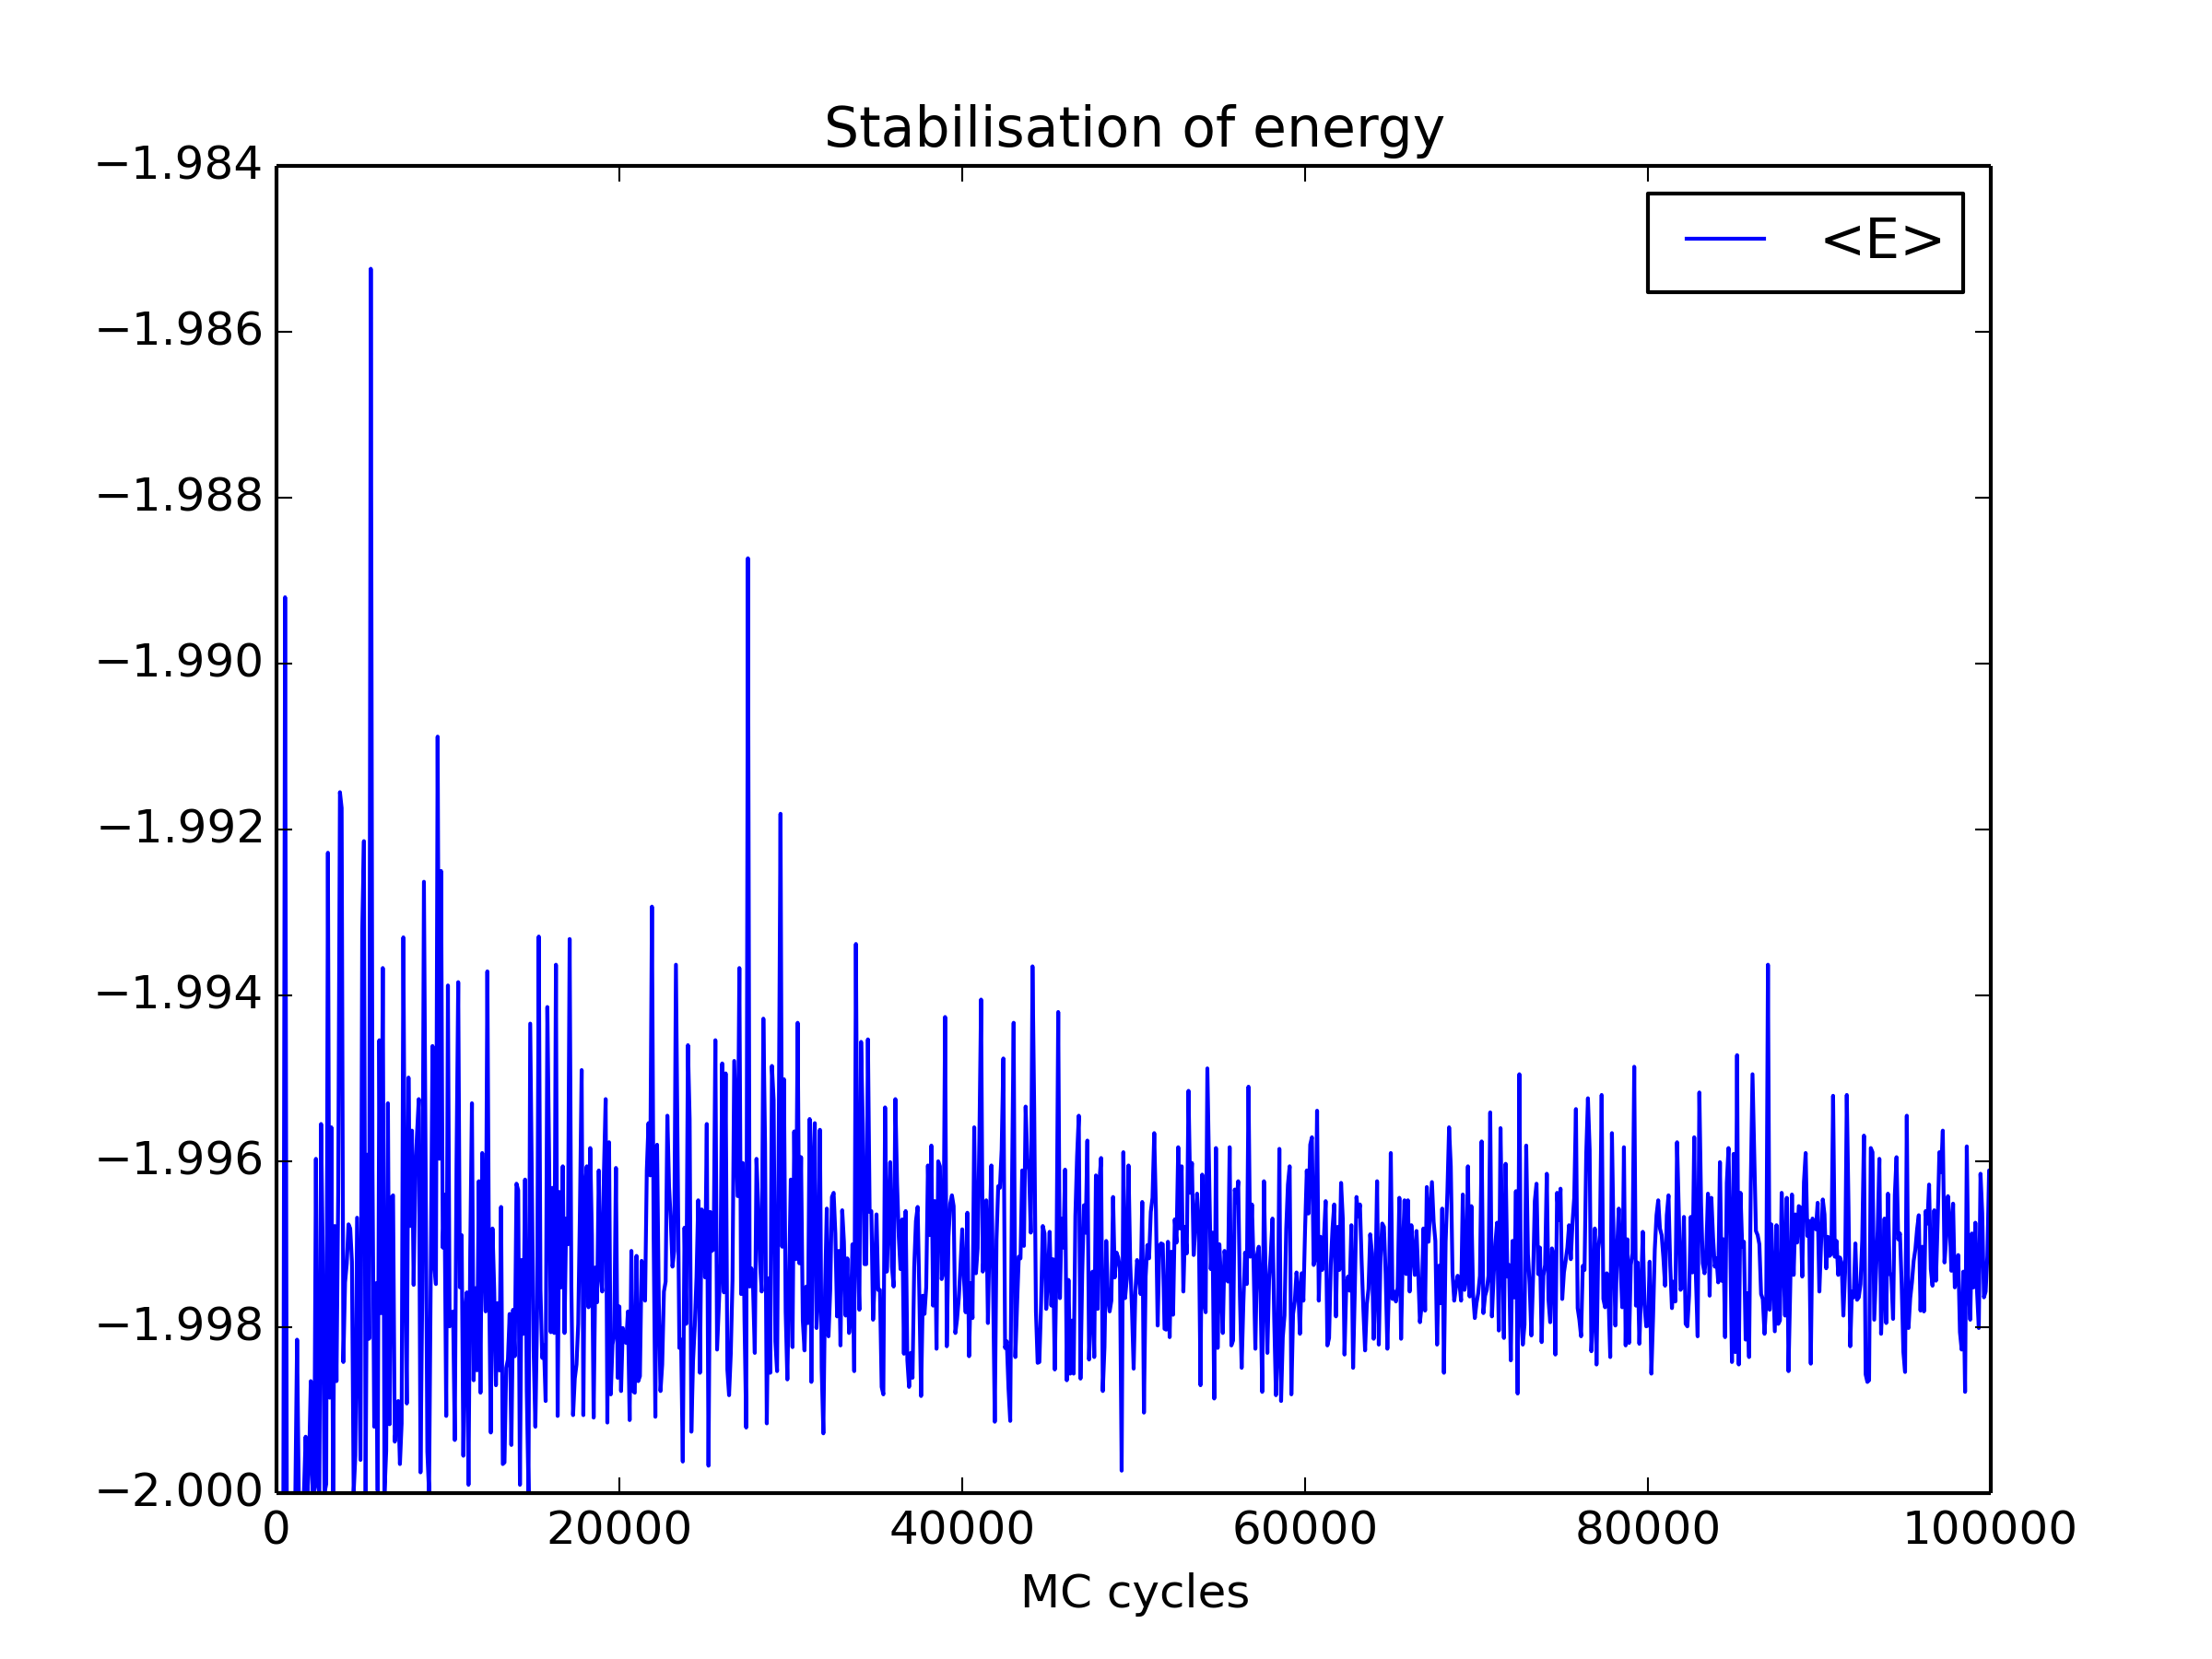
\includegraphics[width=280px]{./plot/L20_1mill.png}
    \caption{Start matrix with all spins up. }
\end{subfigure} \hfill %
\begin{subfigure}{.5\textwidth}
    \centering
    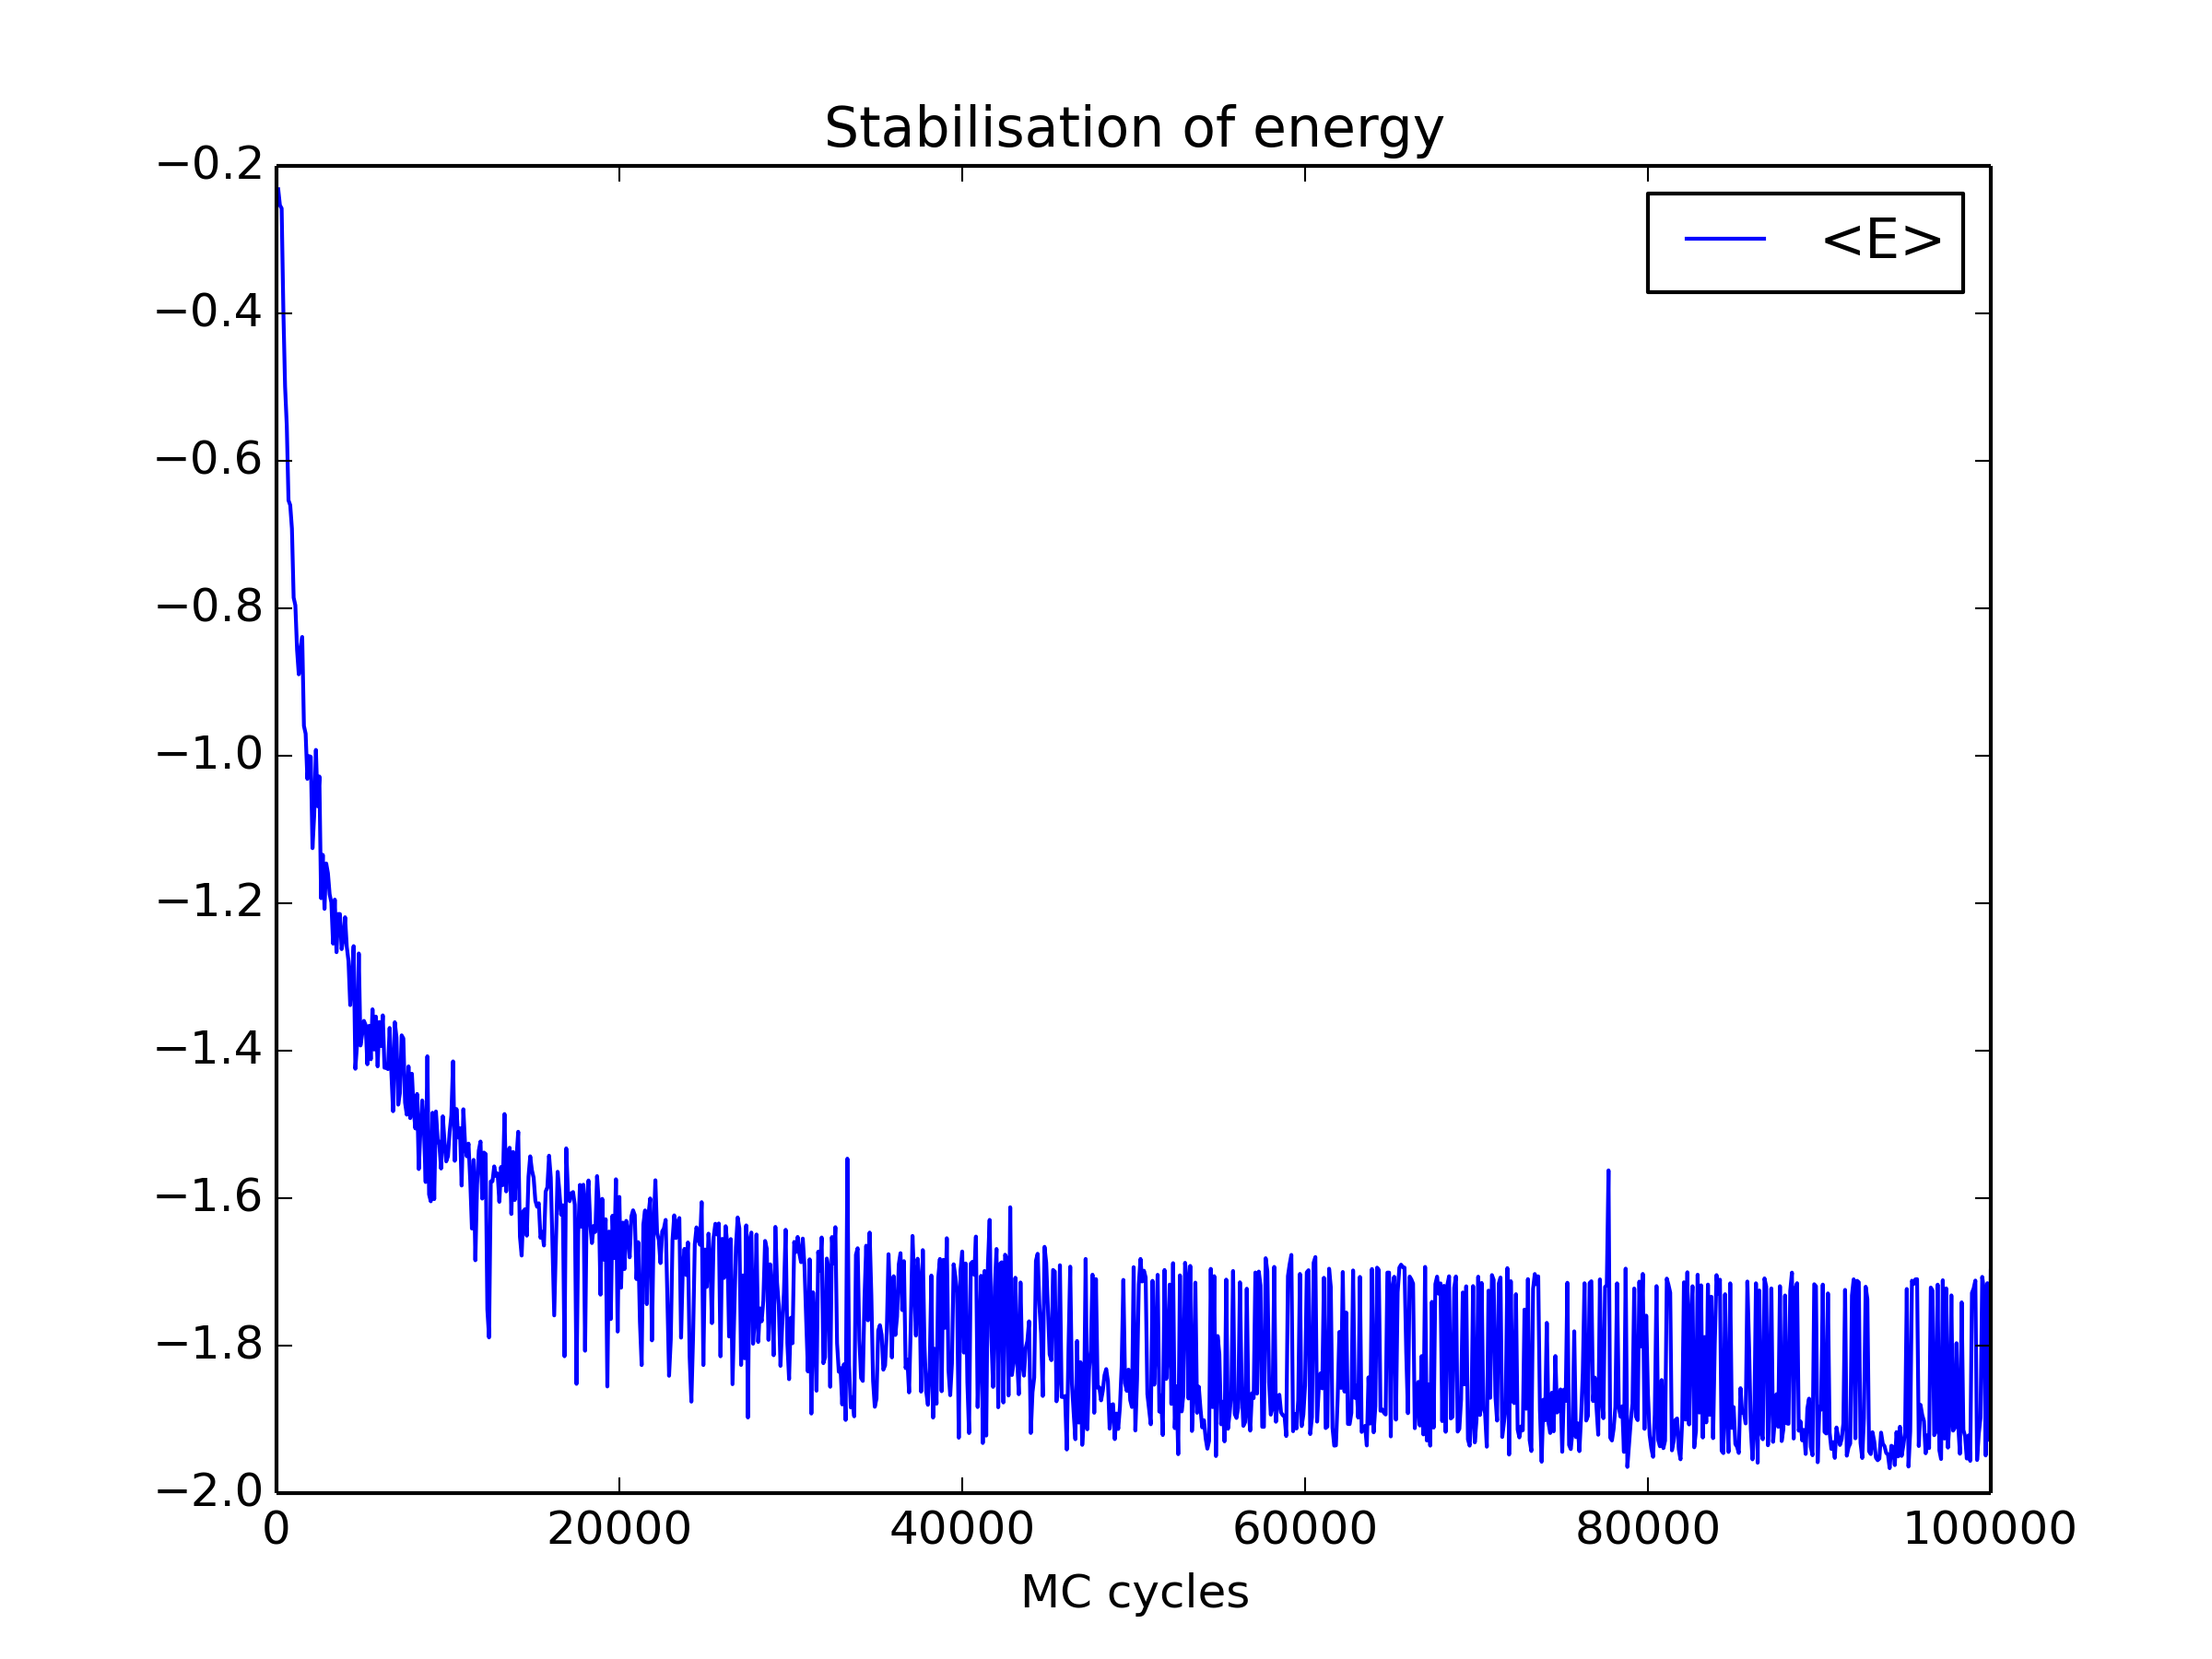
\includegraphics[width=280px]{./plot/random_L20_1mill.png}
    \caption{Start matrix with random spins.}
\end{subfigure}\hfill}}
\caption{: Energy and magnetization plotted against number of Monte Carlo cycles when T = 1.0.}
\label{fig:steady_E}
\end{figure}

If we increase the temperature we excperience that we need several more Monte Carlo cycles to achive the steady state for the energy and the magnetization. Figure \ref{fig:steady_E_highT} shows that we would need around 1 million Monte Carlo cycles for both the random matrix and the matrix with all spins up. An estimate for the actual time it takes to reach equilibrium based on the number of Monte Carlo cycles can be made if we assume that one Monte Carlo cycle equals 1 second. The estimated equilibration times can be found in Table \ref{Tab:equilibration_times}

\begin{figure}
\makebox[\textwidth]{\makebox[1.5\textwidth]{%
\begin{subfigure}{.5\textwidth}
    \centering
    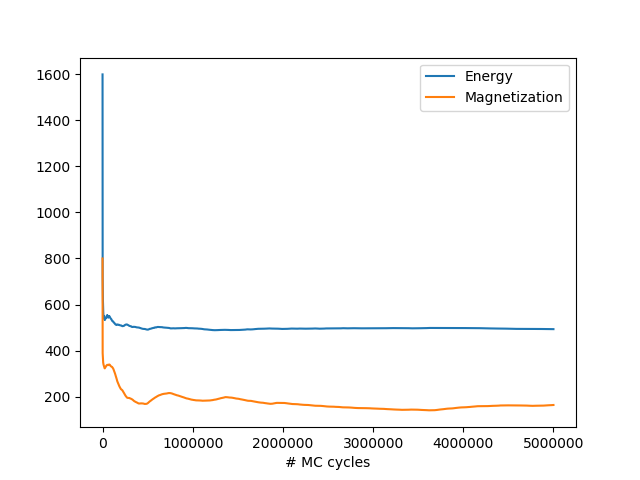
\includegraphics[width=280px]{./plot/L20_5mill_highT.png}
    \caption{Start matrix with all spins up. }
\end{subfigure} \hfill %
\begin{subfigure}{.5\textwidth}
    \centering
    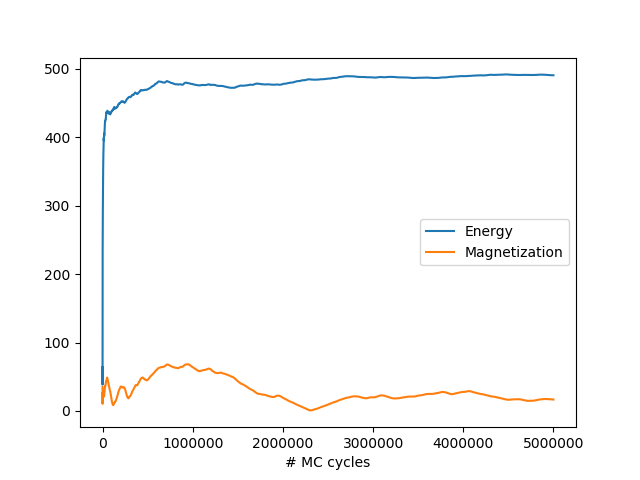
\includegraphics[width=280px]{./plot/random_L20_5mill_highT.png}
    \caption{Start matrix with random spins.}
\end{subfigure}\hfill}}
\caption{: Energy and magnetization plotted against number of Monte Carlo cycles when T = 2.4. }
\label{fig:steady_E_highT}
\end{figure}

{\renewcommand{\arraystretch}{1.5}
\begin{table}[h!]
  \caption{: Estimated equilibration times.}
    \label{Tab:equilibration_times}
    \centering
  \begin{tabular}{c c}
      Matrix & Equilibration time (sec)\\
      \hline
      T = 1.0 in a random spin matrix & 200 000  \\
      T = 1.0 in a matrix with all spins up & $\approx$ 0 \\
      T = 2.4 in a random spin matrix & 1 000 000\\
      T = 2.4 in a matrix with all spins up & 1 000 000\\
    \hline
  \end{tabular}
\end{table}

Figure \ref{fig:flips} and Figure \ref{flips_random} show plots of the total number of accepted configurations as function of the total number of Monte Carlo cycles for respectively a start matrix with all spins up and a start matrix with random spins.

\begin{figure}
\makebox[\textwidth]{\makebox[1.5\textwidth]{%
\begin{subfigure}{.5\textwidth}
    \centering
    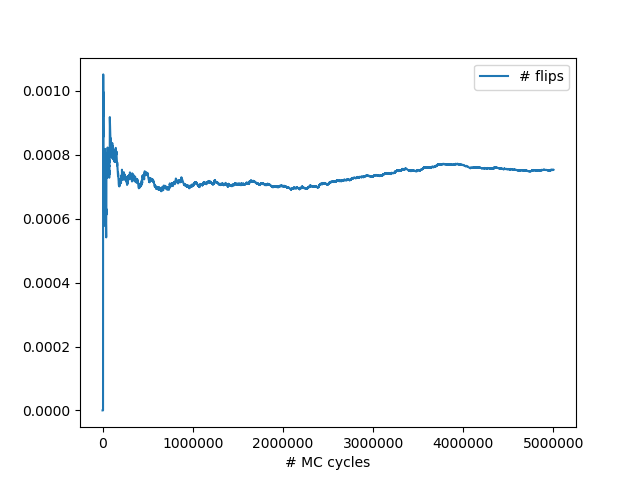
\includegraphics[width=280px]{./plot/number_of_flips.png}
    \caption{T = 1.0}
\end{subfigure} \hfill %
\begin{subfigure}{.5\textwidth}
    \centering
    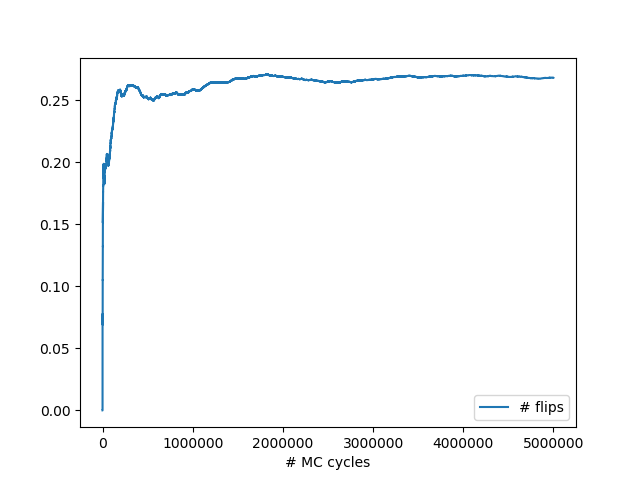
\includegraphics[width=280px]{./plot/number_of_flips_highT.png}
    \caption{T = 2.4}
\end{subfigure}\hfill}}
\caption{: Total number of accepted spinconfiguration as a function of Monte Carlo cycles, for a start matrix with all spins up. }
\label{fig:flips}
\end{figure}

\begin{figure}
\makebox[\textwidth]{\makebox[1.5\textwidth]{%
\begin{subfigure}{.5\textwidth}
    \centering
    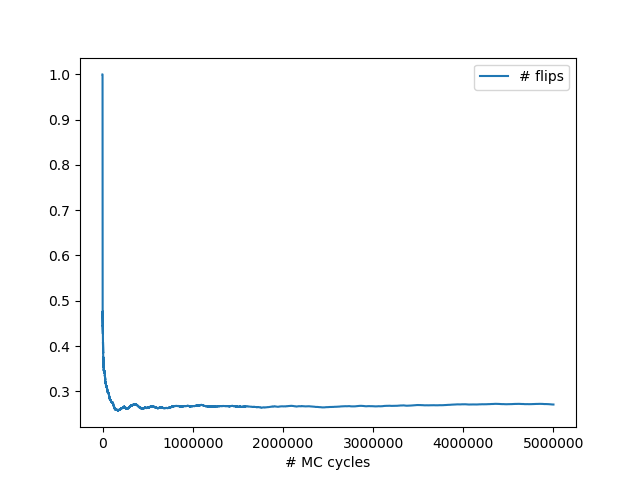
\includegraphics[width=280px]{./plot/random_number_of_flips.png}
    \caption{T = 1.0}
\end{subfigure} \hfill %
\begin{subfigure}{.5\textwidth}
    \centering
    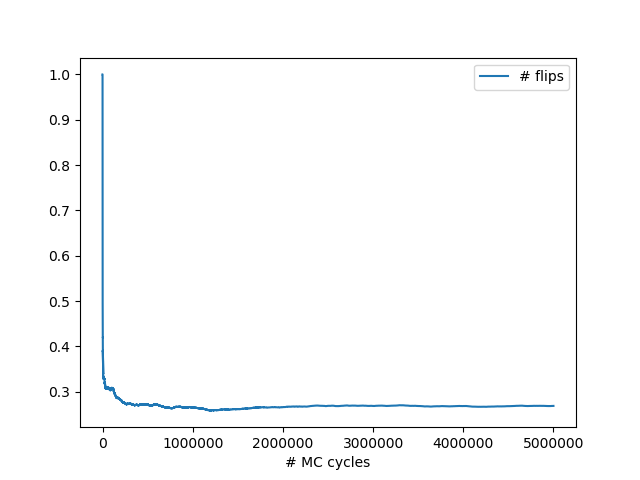
\includegraphics[width=280px]{./plot/random_number_of_flips_highT.png}
    \caption{T = 2.4}
\end{subfigure}\hfill}}
\caption{: Total number of accepted spinconfiguration as a function of Monte Carlo cycles, for a start matrix with all spins up. }
\label{fig:flips_random}
\end{figure}


% d)
The propability distribution for the energy for T = 1.0 and T = 2.4 is shown in figure \ref{fig:propability}.

\begin{figure}
\makebox[\textwidth]{\makebox[1.5\textwidth]{%
\begin{subfigure}{.5\textwidth}
    \centering
    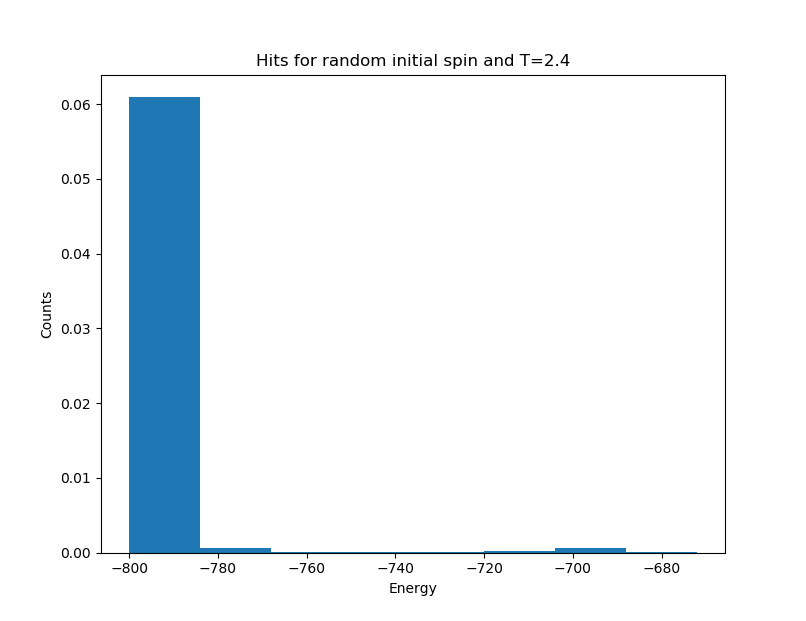
\includegraphics[width=280px]{./plot/histogram_random_lowT.png}
    \caption{T = 1.0}
\end{subfigure} \hfill %
\begin{subfigure}{.5\textwidth}
    \centering
    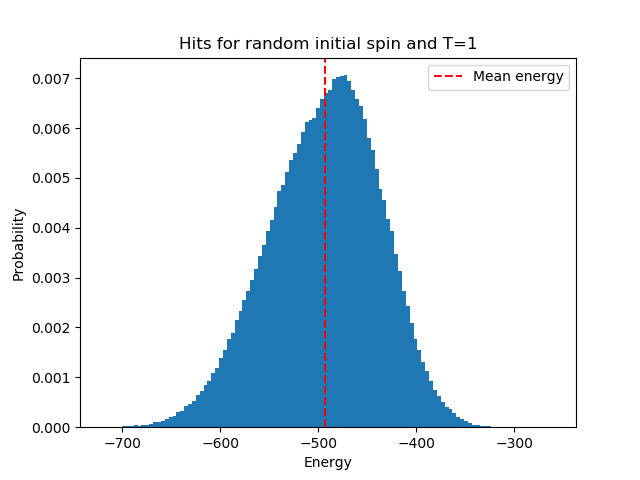
\includegraphics[width=300px]{./plot/histogram_random_highT.png}
    \caption{T = 2.4}
\end{subfigure}\hfill}}
\caption{: Propability distribution for counted energies.}
\label{fig:propability}
\end{figure}


\section{Discussion}

%b) Compare your results with the expressions from a) for a temperature T = 1.0 (in units of kT /J).
%How many Monte Carlo cycles do you need in order to achieve a good
%agreeement?

The numerical value for $<E>, <E^2>$ and $C_v$ for a 2x2 lattice gives a godd compliance to the analytical values. However the numerical values for the magnetization and the susceptibility does not compliance well with the analytical values. The mean magnetization does vary alot more in different calculations because it depends more of how the spins flip. While the energy depends on the square of neighboring spins, the magnetization depends on the sum over all spins, this may be why we excperience different values for the mean magnetization in different calculations.

% c)
From Figure \ref{fig:steady_E} and \ref{fig:steady_E_highT} we see that the energy and magnetization needs a lot less time to stabelize when all of the spins in the lattice have the same configuration and T = 1.0. When we increase the temperature the number of Monte Carlo cycles we need to get a good results also increase. For a higher temperature we can also see that the energy in the system increases. As mentioned above the magnetization is more dependent on the spin configuration in the entire matrix and therefore it will not be as stable as the energy.


%Vi må kommentere Figure \ref{fig:flips} and Figure %\ref{flips_random}

We can see that the variance is incresing with temperature, that is why we get a propability distribution which is more spread out in energies when the temperature is increasing.

\section{Conclusion}
We have

\section{Appendix}

\subsection{Degenerated energies and magnetization}

When calculating the degenerate energies for the case of 2x2, we start with the equation $E_i=-J\sum\limits_{\left<kl\right>}^{2}s_ks_l$\\
The case for all spin up looks like this
\begin{tabular}{c c}
  $\uparrow$ & $\uparrow$\\
  $\uparrow$ & $\uparrow$
\end{tabular}\\

And the equation will be.
\begin{flalign*}
  E_1 &= -J\sum\limits_{<kl>}^{2}s_k s_l\\
  &= -J((s_1 s_2+s_1 s_3)+(s_2 s_1+s_2s_4)+(s_3s_1+s_3s_4)+(s_4s_3+s_4s_2))\\
  &= -J((1+1) + (1+1) + (1+1) + (1+1))\\
  E_1 &= -8J
\end{flalign*}
The reason why the same interaction is included several times is because of the unit cell repeating itself to infinity in both x and y derection. Therefore the $s_1$ will interact with $s_2$ and $s_3$ inside the unit cell, and $s_2$ and $s_3$ "outside" the unit cell.

The magnetization is defined as
\begin{flalign*}
  M_i=\sum_{j=1}^{N} s_j
\end{flalign*}
which sums over all spins for a given configuration $i$. For the same spinconfiguration as above this gives:
\begin{flalign*}
  M_i=\sum_{j=1}^{4} (1 + 1 + 1 +1) = 4
\end{flalign*}

\subsection{The partition function}
When we known the values for all the degenerate energies we can calculate the value of the partian function.
\begin{flalign*}
  &z = \sum\limits_{i=1}^{2^n}e^{-\beta E_i}\\
  &\text{In out case we have $n=4$ since we have a 2x2 lattice.}\\
  &z = \sum\limits_{i=1}^{2^4}e^{-\beta E_i}\\
  &z = e^{-\beta E_1}+e^{-\beta E_2}+\hdots+e^{-\beta E_16}\\
  &z = e^{8 \beta J}+4e^{- \beta \cdot 0} + 2e^{-8 \beta J} + 4e^{-\beta \cdot 0} + 4e^{-\beta \cdot 0} + 4e^{-\beta \cdot 0} + e^{8 \beta J}\\
  &z = 2e^{8 \beta J} + 2e^{-8 \beta J} + 16
\end{flalign*}

\subsection{Expectationvalues for the energy}
This gives us the ability to calculate the expectationvalue of the energy $\left<E\right>$

\begin{flalign*}
  \left<E\right> &= \sum\limits_{i}^{2^n}\frac{E_i e^{-\beta E_i}}{z}\\
  &\text{We know we have several energyvalues which is zero. If we do not write these we get}\\
  &= \frac{-8Je^{8\beta J} +2\left(8Je^{-8 \beta J} \right) + \left(-8J\right)e^{8\beta J}} {2e^{8 \beta J} + 2e^{-8 \beta J} + 16}\\
  &= \frac{16J\left(e^{-8\beta J}- e^{8 \beta J} \right) }{2 {\left(e^{8 \beta J} + e^{-8 \beta J} + 8 \right)} }\\
  &= 8J \frac{e^{-8\beta J}- e^{8 \beta J}}{e^{8 \beta J} + e^{-8 \beta J} + 8}
\end{flalign*}

Thus
\begin{flalign*}
  \left<E\right>^2 &= \left( 8J \frac{e^{-8\beta J}- e^{8 \beta J}}{e^{8 \beta J} + e^{-8 \beta J} + 8} \right)^2\\
  &= 64J^2 \frac{\left(e^{-8\beta J} - e^{8\beta J} \right)^2 }{\left(e^{8\beta J} + e^{-8 \beta J} + 8 \right)^2 }\\
  &= 64 J^2 \frac{e^{-16\beta J} + e^{16 \beta J} + 2}{e^{16\beta J} + e^{-16\beta J} + 16e^{-8\beta J} + 16e^{8 \beta J} + 66 }
\end{flalign*}

At the same time we calculate $\left<E^2\right>$

\begin{flalign*}
  \left<E^2\right> &= \sum\limits_{i}^{2^n}\frac{E_i^2 e^{-\beta E_i}}{z}\\
  &= \frac{64J^2e^{8\beta J} + 2\left(64J^2e^{-8\beta J}\right) + 64J^2e^{8\beta J}}{2e^{8 \beta J} + 2e^{-8 \beta J} + 16}\\
  &= \frac{128J^2e^{8\beta J} + 128J^2e^{-8\beta J}}{2e^{8 \beta J} + 2e^{-8 \beta J} + 16}\\
  &= 64J^2\frac{e^{8\beta J} + e^{-8\beta J}}{e^{8 \beta J} + e^{-8 \beta J} + 8}
\end{flalign*}

\subsection{Expectationvalues for the magnetization}
The absolute value of the mean magnetization is given by
\begin{flalign*}
  \left<|M(T)|\right> = \frac{\sum \limits{_i^{2^4}} |M_i| e^{-\beta E_i}}{z}
\end{flalign*}
and can be calculated by using the values for the energy and the magnetization from Table \ref{Tab: EogM}:

\begin{flalign*}
  \left<|M(T)|\right> &= \frac{4e^{8\beta J} + 2\cdot4 + 0\cdot4 + 0\cdot2 + |-2|\cdot4 + |-4|e^{8\beta J}}{z}\\
  \left<|M(T)|\right> &= \frac{8e^{8\beta J} + 16}{2e^{8 \beta J} + 2e^{-8 \beta J} + 16} = \frac{4e^{8\beta J} + 8}{e^{8 \beta J} + e^{-8 \beta J} + 8}
\end{flalign*}

We also have that
\begin{flalign*}
  \left<|M(T)|^2\right> &=  \frac{\sum \limits{_i^{2^4}} |M_i^2| e^{-\beta E_i}}{z}\\
  \left<|M(T)|^2\right> &= \frac{32e^{8\beta J} + 32}{2e^{8 \beta J} + 2e^{-8 \beta J} + 16} = 16\frac{e^{8\beta J} + 1}{e^{8 \beta J} + e^{-8 \beta J} + 8}
\end{flalign*}

\subsection{Heat Capacity}
We the expectationvalues to calculate the variance for the energy
\begin{flalign*}
  \sigma^2_E &= \left<E^2\right> - \left<E\right>^2\\
  &= 64J^2\frac{e^{8\beta J} + e^{-8\beta J}}{e^{8 \beta J} + e^{-8 \beta J} + 8} - 64 J^2 \frac{e^{-16\beta J} + e^{16 \beta J} + 2}{e^{16\beta J} + e^{-16\beta J} + 16e^{-8\beta J} + 16e^{8 \beta J} + 66 }
\end{flalign*}

When this is known we can also calculate the heat capasitace.
\begin{flalign*}
  C_v &= \frac{\sigma^2_E}{k_BT^2}\\
  &= \frac{64J^2}{k_BT^2}\left[\frac{e^{8\beta J} + e^{-8\beta J}}{e^{8 \beta J} + e^{-8 \beta J} + 8} -  \frac{e^{-16\beta J} + e^{16 \beta J} + 2}{e^{16\beta J} + e^{-16\beta J} + 16e^{-8\beta J} + 16e^{8 \beta J} + 66 }\right]
\end{flalign*}


\subsection{Susceptibility}
The variance for the absolute value of the mean magnetization is given by:
\begin{flalign*}
  \sigma_{M}^2 &= \left<|M(T)^2|\right> - \left<|M(T)|\right>^2\\
  \sigma^2_M &= 16 \frac{e^{8\beta J} + 1}{e^{8 \beta J} + e^{-8 \beta J} + 8} - 16\frac{e^{16\beta J} + 4e^{8\beta J} + 4}{e^{-16\beta J} + e^{-16\beta J} + 16e^{-8\beta J} + 16e^{8 \beta J} + 66}
\end{flalign*}

We then calculate the susceptibility $\chi$ which is given by $\chi = \sigma_M^2/k_BT$, so

\begin{flalign*}
  \chi = \frac{16}{k_BT} \left[{\frac{e^{8\beta J} + 1}{e^{8 \beta J} + e^{-8 \beta J} + 8} -\frac{e^{16\beta J} + 4e^{8\beta J} + 4}{e^{-16\beta J} + e^{-16\beta J} + 16e^{-8\beta J} + 16e^{8 \beta J} + 66}}\right]
\end{flalign*}

\section{Bibliography}


\end{document}
